\documentclass[12pt]{article}
\usepackage[utf8]{inputenc}
\usepackage{titling}
\usepackage{amssymb}
\usepackage{geometry} 
\geometry{a4paper}              
\usepackage{graphicx}
\usepackage{hyperref}
\usepackage{wrapfig}
\usepackage{float}
\usepackage{comment}
\usepackage{hyperref}
\usepackage{listings}
\usepackage{tabu}
\usepackage{longtable}
\usepackage{color}
\usepackage[table, svgnames]{xcolor} 
\usepackage{array}
\usepackage{cellspace}
\usepackage{minted}

\usepackage[
backend=biber,
sorting=ynt
]{biblatex}
\usepackage{etoolbox}

\addbibresource{my.bib}
\renewcommand*\contentsname{Table of Contents}

 \AtBeginEnvironment{tabular}{\rowcolors{1}{\ifnumless{\rownum}{2}{DarkSeaGreen!40}{white}}{}}
\renewcommand{\arraystretch}{2}

 
\begin{document}

\begin{center}
    ~\\ 
    ~\\ 

    
\includegraphics[width=10cm]{logom.png} 
    ~\\ 
    ~\\ 

    ~\\ 
    ~\\ 
    ~\\ 
    \Huge JVM stack-trace debugging in production systems \\
    ~\\ 
    ~\\ 
        ~\\ 

    \large Student\\ 
    \Large Adrian M. Nenu\\  
    ~\\    
    ~\\ 

    \large Supervisor\\  
    \Large Dr. Caroline Jay
    ~\\ 
    ~\\    
    ~\\ 
    ~\\ 
    ~\\ 

    \large May 2017
\end{center}

\thispagestyle{empty}

\newpage

\begin{center} {\LARGE Abstract} \end{center}

~\\
~\\


The Java Virtual Machine has become one of the most popular frameworks for running code in a cross-operating-system and performance-aware fashion, aspects of paramount importance in modern software.

With the acknowledgement that no software, no matter how well planed and executed, is bug-less and the awareness that developers must expect even random errors which would be incredibly difficult to predict, perhaps errors specific to running an app in a distributed environment, programs are moving towards providing self-healing behaviours and interfaces which can ease the debugging effort, especially in production systems.

One more aspect of modern software development is the advent of open-source communities. An individual software engineer can accomplish today what entire teams could execute in the same period of time in the past by taking advantage of the building blocks offered by the community at large and contributing back with his own changes and ideas. 

In this report the techniques available to efficiently analyse the behaviour of the Java Virtual Machine and how debugging software can take advantage of them (even in production environments) are presented. A multiple-component system has been developed to allow the debugging of JVM based software in the following way:

The focus point is being able to obtain a relevant slice of the state of the JVM at the time when an error occurs in the system. We will look upon an error as any exception which the JVM detects and capture the values of relevant variables used in the code inside the methods which are part of the stack-trace of these exceptions. This will provide us with a contextual approach to debugging, providing the ability to discover whether the issue at hand has developed due to an input or programming error.

Many concerns have arisen with this approach, such as the recursive potential of objects in the JVM referencing each other, secure storage of captured data and avoiding recording the same exceptions across apps deployed in multiple instances, which we will discuss.

The code is made available to the open-source community as interest has been manifested by enterprises for an openly licensed tool which they can customise to their own specific requirements without being under intellectual property regulations.

\newpage

\begin{center} {\LARGE Acknowledgements} \end{center}

~\\
~\\

Firstly, I would like to thank my supervisor, Dr. Caroline Jay, for her continued support of the project and for always making sure it stayed on track regardless of my high-level goals which has allowed for the core to be developed first and then for other features to be built upon it.

Secondly, I would like to thank the professors and professionals who have contributed their ideas and feedback in order to establish the requirements and need for such a project. 

A thank you for the students who have helped evaluate and improve the ideas explored in this report is also in order.

Last, but not least, I thank my parents for giving me the opportunities to reach my goals.

\newpage

\tableofcontents

\newpage


\listoffigures


\newpage

\listoflistings


\newpage

\section{Introduction}

\subsection{Overview}

The aim of this project is to build a JVM debugging tool able to detect errors and capture snapshots of the state of the system with minimal performance impact, with the potential of running even on production systems without compromises on stability or resource usage.

The Java Native Interface a and JVM Tool Interface, providing low-level entry and event capturing points into the state of the Java Virtual Machine, are used to read the heap and extract useful data that can help developers construct a context-aware picture of the situation at the time at which errors have taken place.

The main part of the tool is represented by a library to which this report refers to as the agent, that can latch itself to any JVM at start-time or run-time and accomplish the desired behaviour of capturing a slice of the values of variables when an exception takes place.

Concerns such as secure storage of data and code-base code, which could be used to overlay captured variable data on, are explored. 

One of the most challenging aspects has been communicating with the JVM using the previously mentioned interfaces. Many scenarios have had to be handled in order to parse the heap and recover all relevant data that might beof interest such as static and instance variables, objects referencing other objects, custom classes and others, all of which have brought their own complications.

The cross-operating compilation aspect of a native library has also brought a certain level of complexity, for example the threading libraries and JDK package which are different for say UNIX and Windows systems.

\subsection{Motivations}

There is an uncountable amount of logging libraries and JVM heap monitors and dumpers, such as the well known tool jvisualvm which can be used to debug the JVM generally with a very noticeable impact on its performance \cite{jvisualvm}. However, specialised open-source tools for capturing only the objects of interest on a stack-trace, preferably built for speed and performance in order to enable usage in production systems are available only in a Platform as a service way.

A number of industry representatives manifested interest in an open source tool to cover this need and emphasised the fact that similar providers hold their software under intellectual property license.

\subsection{Aims}
The main aim is building an open-source minimum viable product native agent which can accomplish the task of handling and capturing the values of variables from the JVM heap (object tree) when exceptions occur at runtime with minimal performance impact on the JVM. 

A secondary aim is to provide a web dashboard for visualising and exploring the captured data through an user-friendly interface.

And the final high-level aim is to research the different issues a system of this kind may face and their potential solutions even if they might be out of the scope of the project given the implementation time and resource constraints.

\subsection{Context}
This section presents general definitions of the the most important concepts used across this report. The reader who is familiar with these definitions may skip this part as it does not cover aspects specific to this project.

\subsubsection{Java and the JVM}
Since its initial introduction in 1995 \cite{javaPerfJVM}, the Java Virtual Machine, referred to henceforth as the JVM, has gained popularity up to the enterprise level. With a Just in time compiler, cross-operating-system running ability, a lot of attention to backward compatibility and memory management via the garbage collector, the JVM has brought about the introduction of other programming languages than Java as well, such as Scala and Clojure \cite{jvmLangs}. Apps developed in any such JVM based languages could be a potential client of the tool developed through in this project.

Java (and other bytecode compatible languages) is transformed into bytecode which the JVM can run on any system able to run the JVM itself. The JVM takes care of memory management and many other performance and security aspects of the application. The Just In Time compiler (JIT) converts bytecode into machine dependable code (executable by the CPU) on a per-need basis, at run-time \cite{javaCompilerJVM}. This is what gives its main cross-operating-system and performance advantages. Moreover, the JVM offers very good interfaces for accessing its state at runtime which allows us to to build tools such as the one aimed by this project. Some of these interfaces are explored in the following subsections.

\subsubsection{The Java Native Interface - JNI}
The Java Native Interface, henceforth referred to as the JNI, allows code running inside of the JVM to interact with external libraries built in other programming languages. Agents using JNI calls can be created in languages such as C, C++ or even straight assembly \cite{javaPerfJVM}.

The JNI could be used to alter the behaviour of applications, but this project mainly explores the observing capabilities it allows into the JVM state.

\subsubsection{Exceptions and stack-traces}
For the scope of this report, stack traces represent the sequence of stacked functions down to the point when an exception takes place. They allow us to track the execution path to the exception triggering block of code \cite{stacktrace}.

The stack-trace is divided into multiple entries, in this case methods, called frames. 

The end product of this project is meant to detect exceptions and, by going through each frame, capture the values of locally defined and statically available variables.

\begin{listing}[H]
\begin{minted}[breaklines=true]{c}
Exception in thread "main" java.lang.NullPointerException
        at com.demo.project.Book.getTitle(Book.java:15)
        at com.demo.project.Author.getBookTitles(Author.java:30)
        at com.demo.project.Bootstrap.main(Bootstrap.java:13)
\end{minted}
\caption{Example of a JVM stack-trace}
\end{listing}

\subsubsection{The JVM Tool Interface - JVMTI}
The Java Virtual Machine Tool Interface, henceforth referred to as the JVMTI, can be used to monitor and debug a JVM \cite{jniwhatis}. It offers the ability to subscribe to a number of events out of which we are concerned with only one: jvmtiEventException \cite{jnievents}.

Given an object, the JVMTI can be used to obtain its properties and fields.

The JVMTI functions use JNI references to identify objects  (jobject and jclass) \cite{jniref}.

The JVMTI and JNI are comprehensive tools for studying the behaviour of the JVM and once understood can be used to built useful debugging tools which can really ease the process of identifying the source of problems.


\newpage



\section{System design choices}
\subsection{Overview}


The overall system needed to accomplish the following high-level tasks
\begin{itemize}
  \item Detect exceptions and extract values of variables on the stack-trace
  \item Store the captured data for later analysis
  \item Provide a useful visualisation of extracted data
\end{itemize}

With these primordial functions in mind, four main components evolved
\begin{enumerate}
  \item An Agent attached to every JVM instance which can capture the data
  \item An API to which the Agent send the data
  \item A Database with which the API engine can interact to store and read data
  \item and a Dashboard Portal that connects to the API and provides a view-port into the collected and processed data
\end{enumerate}

A micro-service pattern has been considered when designing this service suite \cite{microservices}. All of the components are built in different programming languages and can be deployed independently as long as the versions in production have common communication interfaces or are otherwise backward compatible with each other.

The agent itself is a micro-service towards the JVM it is observing. It runs as a separate process and it can be attached at any point in the lifetime of the JVM.

\begin{figure}[H]
  \centering
    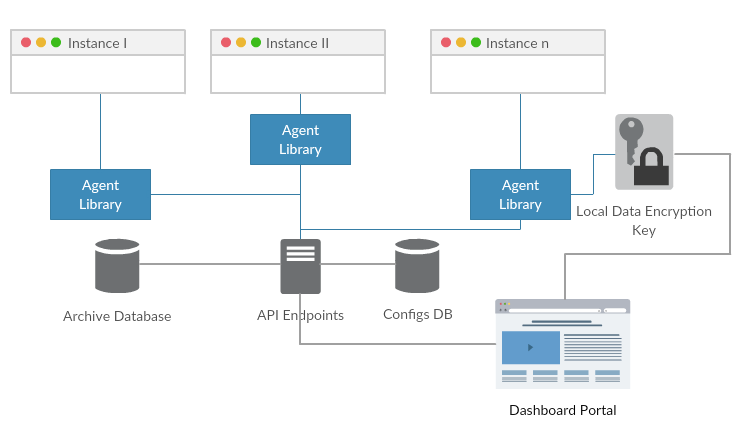
\includegraphics[width=\textwidth]{initial-design.png} 
  \caption[Initial system design diagram]{The initial system design, before the start of implementation.}

\end{figure} 

The initial system design included a configuration database which would allow the user to configure properties of how the agent behaved through the Dashboard Portal. Moreover, it factored in the way encryption may be accounted for. As we shall see in the next section, these parts have been excluded from the core for the purpose of finishing a base version before further improvements are considered.

\subsection{Revised and final system components} 

\begin{figure}[H]
  \centering
    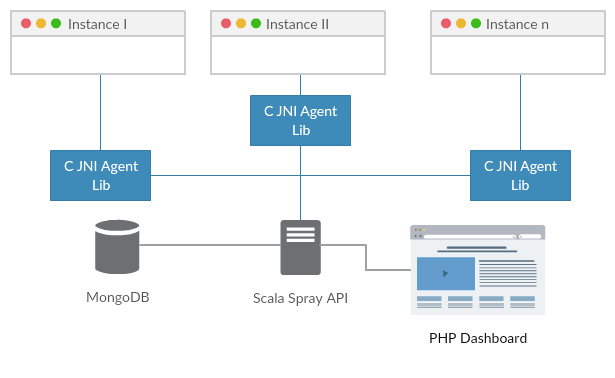
\includegraphics[width=\textwidth]{end-design.png} 
  \caption[Revised system design diagram]{The revised system design, as an artefact after the end of implementation.}

\end{figure}

After going through a few revisions in the lifetime of the project, the final system has been implemented following this design:



The reasons why each of the components has been developed in the mentioned programming language are explored in the next section.

\subsection{Agent Library}
\subsubsection{Overview}

This component is focused on using the JNI and JVMTI to obtain data from the JVM. More specifically, its purpose is to capture a relevant slice of the variable-tree and use the JVMTI exception callback to decide when to record this data. One of these cases being when an exception has been detected.

The agent must have access to explore the stack-trace and the ability to match variable data to the methods present on the stack trace.

\subsubsection{Technology choice}

\begin{figure}[H]
  \centering
    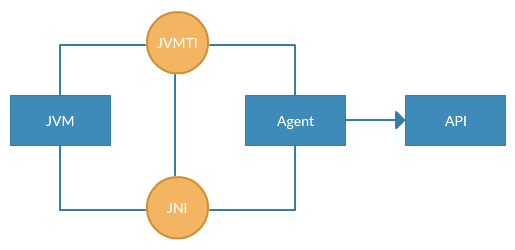
\includegraphics[width=\textwidth]{jvmti.png} 
  \caption[JVMTI and JNI provide access for the Native Agent to the JVM]{JVMTI and JNI provide access for the Native Agent into the JVM}

\end{figure} 

Two main options were considered: a Java agent versus a Native agent.

A Java agent cannot access low-level aspects of the JVM with as much ease as a native one and it cannot run as a separate process which means that if it crashes it crashes the JVM as well. Moreover, because the Java agent becomes part of the JVM, it has impact on the garbage collection and JVM performance, possibly impacting its behaviour in unwanted ways and altering results of other tools the user may be using to analyse resource usage of the app \cite{javavsnativetaki,javavsnativetdyna}.

There are many libraries already built for Java based agents, such as Javaassist \cite{javassist} and ASM \cite{asm}, but their main goals is dynamic bytecode manipulation and given the aims of the project, a native mainly read-only agent made more sense.

A native agent would also be loaded before the JVM loads any classes and stopped after the JVM has wrapped everything up, while the Java based agent is loaded at a later stage in the lifetime of the JVM \cite{javavsnativetdyna}.

The Instrumentation package to which a Java agent would have access to is only for the instrumentation functionality of the JVMTI \cite{jvmtiInterface}.

A native agent has unrestricted access to the lowest level of instrumentation and can most efficiently dig deep into the depths of the JVM. By doing its own memory allocations in the shared memory outside of the managed heap, it allows for a small overhead and no impact into JVM garbage collection time.

The native access has direct native access to the JNI and JVMTI.

\subsubsection{Conclusion}
A native agent implementation using the JNI and JVMTI interfaces is the choice that best matches the scope of this project. 

\subsection{Database}
\subsubsection{Overview}
The database engine needs to be able to handle concurrent writes but not particularly to the same object as once the data for a stack-trace is recorded, it is never updated.

Advanced filtering is also not very important. Simple queries would be enough to serve the purposes of the current system, such as filtering by the originating app.

At this prototype level, a preference to a flexible structure for stored entries is preferred.

\subsubsection{Technology choice}
There were many approaches which could be taken for the log storage engine. Specialised tools for storing log-like data could have been used, such as Logstash \cite{logstash}, which would provide good interfaces for analysing the data and handling concurrent writes.

Graph-based database engines were also a consideration and might provide specific advantages for future versions of this product, when its ability to scale into handling multiple instances of apps improves.

However, more traditional engines were considered as the main choices in order to easily provide storage for the user, configuration and session data through the same engine.

While servers such as MySQL and MSSQL would have offered better querying capabilities and would be the better choices when storing entities which relate to one another to avoid duplication, NoSQL-like engines matched the project's iterative changing requirements better.

MongoDB is a well documented and flexible engine with adaptors built in most popular programming languages including the choices made for this project. 

\subsubsection{Conclusion}
MongoDB was picked based of familiarity, documentation and flexibility.

\subsection{API}
\subsubsection{Overview}
An Application Programming Interface, referred to as the API, will be provided, sitting at the centre of the system. The Agents communicate with this service to store data and the Dashboard accesses the service on order to obtain it.

Authentication for the dashboard will be done via a token-based session management approach and the agents will use an API key and App key to relate the specific data they register to a specific user configured app.

Currently, multiple instances of the same app would use the same App key.

\subsubsection{Technology choice}
A RESTful HTTP API design \cite{rest} has been used as the particular kind of usage we are in scope of did not need a continuous connection or server to client communication such as say Sockets could accommodate. Moreover, the API and App keys provide a sufficiently secure level of authentication for each request.

But Sockets could be an interesting choice in the future for agents to locally communicate with one another, especially agents attached to different instances of the same app, which could avoid recording the same stack-traces by locally exchanging information.

There are numerous frameworks for most programming languages which can serve as an API base. As such, it is very hard to attempt to select the very best choice and the selection process ended up considering aspects such as developer familiarity with the programming language.

NodeJS and Python were the initial candidates. However, they were both outranked by Scala for the same reason, which is the lack of a default typed environment (strict definitions for variables and compile-time detection of potential type-related mistakes) \cite{scalaVSjsRH}. The advantage of a typed language out-weighted the shorter development time.

NodeJS, for example, has Typescript as a way to work-around this problem.

Scala has been steadily gaining terrain in the enterprise world and is trusted by developers. Given also that the kind of data meant to be recorded (log-like) is often never altered it is ideal for a functional programming language.

One other interesting part about having a JVM (Scala) based component would be the ability to run the end product (the agent) on it. However, the project has not reached this phase at this time.

\subsubsection{Conclusion}
The Scala Spray framework combined with SBT for dependency management ended up being the technology choice for this component.

\subsection{Dashboard Portal}
\subsubsection{Overview}
The purpose of this component is to allow the user actor to view data extracted by the agent in an intractable and friendly manner.

The dashboard talks to the API to create user sessions and obtain data. It would likely have to do some processing of the data itself in order to extract further information and the frontend might have to be encryption-aware in order to use local decryption keys to render protected data.

\subsubsection{Technology choice}

For this prototype and considering how little work the dashboard had to do, the decision to use PHP as the backend was made.


\subsubsection{Conclusion}
A Model-View-Controller framework named FuelPHP was used for separation of concerns and the in-built HTTP request framework handled the communication with the API.

The Twitter Bootstrap framework was used as a start for the design and multiple libraries can provide additional functionality such as encryption and decryption.

\newpage

\section{Implementation}

\subsection{Methodology}

Due to the many initial unknowns and research-driven approach influencing the system design, an Agile mind-set was taken from the start to support changing requirements and iterative working releases.

This proved really useful as many decisions have had to be made after the implementation began and a few compromises have happened, which can be seen from the system design section.

Requirement gathering and the development of testing scenarios also took an Agile approach. Due to the technical aspect of the app, it was easier for users to drive the development after they were able to use the initial version on their own. This has meant that many requirements were obtained after the first iteration finished.

As presented in the System design section, a number of user stories were thought of mainly from the perspective of the Dashboard and were used to drive the development of the entire system. 

\subsection{JNI/JVMTI Agent Library}
For the purpose of gaining performance, not many unneeded libraries have been used. A small logging library has been built from scratch and handles only console output if enabled.

After the heap is reconstructed in the internal data-structure, an XML is built and sent to a thread pending delivery to the API engine.

Handlers have been coded to process the different kinds of primitives and objects that programmers can create in the JVM. Many different edge cases have stood out during research and testing, such as the difference between static and instance fields.

\subsubsection{Requirements on the JVM app owner side}
To deliver any of its promises, the agent requires the Java app to be built using either the defaults for the javac -g option or javac -g:lines,vars. This lets the compiler know that it should also record useful debugging information in the .class files, such as the local variable names \cite{javac}.

Local variables names and line numbers are recorded by default if no -g is specified.

\subsubsection{Mapping primitive, array and object types}

A hashmap data structure based around the object id is created on the native agent side as a mid-transition-point between the JVM heap and the construction of the message sent to the API.

The unique (per exception) object id used to identify an object is obtained using the JVMTI.GetObjectHashCode method which guarantees the returned integer hashcode is different for all objects across their lifetime \cite{GetObjectHashCode}. 

Every single variable is represented in the following data-structure on the agent side regardless of its properties:

\begin{listing}[H]
\begin{minted}[breaklines=true]{c}
struct VarHolder {
  int object_id;
  char * name;
  char * signature;
  char * generic;

  char * value;
  int array_length;
  bool is_static;

  int field_count;
  VarHolder * fields;
}
\end{minted}
\caption{Variable wrapper on the Agent side}
\end{listing}

The code is show so that the reader can build a mental-model of how the system works behind the scenes.

The fields list represents in the case of
\begin{itemize}
  \item an array, each entry held within
  \item an object, each static and non-static field
\end{itemize}

To reduce the complexity of the code needed to handle the processing of variable types, the value/contents of objects (non-primitive variables), where they are not null, is currently established by calling the .toString method using the JNI.CallObjectMethod \cite{jniMethod}. Primitives can be parsed from string into their original format via later processing based on their recorded type.

~\\

The following table defines the mapping used \cite{jniTypes}.

\begin{listing}[H]

\begin{center}
    \begin{tabular}{ |l|l| }
      \hline
        Type Signature & Java Type \\
      \hline
      Z & boolean \\
            \hline

      B & byte \\
            \hline

      C & char \\
            \hline

      S & short \\
            \hline

      I & int \\
            \hline

      J & long \\
            \hline

      F & float \\
            \hline

      D & double \\
            \hline

      L fully-qualified-class & Object / Custom class \\
            \hline

      {[} type & Array of type \\
      \hline

    \end{tabular}
\end{center}

\caption{Mapping type signature to java types}
\end{listing}

All the types before L are considered to be a primitive type. 

\subsubsection{Parsing variable contents recursively}

The following pseudo-code explains on a very high-level how the agent obtains the values it needs to represent the state of each frame/method/stack-entry of a stack-trace:

\begin{listing}[H]
\begin{minted}[breaklines=true]{c}
function to processVariable given var
    if var is a primitive
        handle value according to type 
    if var is an array
        for each entry in var.elements
            processVariable (entry)
    if var is an object
        for each field in var.fields
            processVariable (field)

function to processStackTrace given stack-trace           
    for each frame in stack-trace
        stackLocalVars <- local variables of current frame
        for each var in stackLocalVars
            processVariable (var)
        staticVariables <- static variables of current frame object used in the frame
        for each var in staticVariables
            processVariable (var)
\end{minted}
\caption{High-level pseudo-code for obtaining values of variables on a stack-trace}
\end{listing}

The actual code under the processVariable function changes depending on whether the variable is static or local.

There are a few cases to consider when dealing with variables
\begin{itemize}
  \item Are they locally defined?
  \item Are they static variables? 
  \item Are they arrays?
  \item Are they objects?
\end{itemize}

If we are dealing with objects then the agent will explore all the fields defined for them. The JVMTI provides a method named GetClassFields which is used for that purpose. Each field is then handled in the same way recursively, for example are any of the fields a primitive, an object or an array?

The same pattern is used for handling arrays, only that the fields are considered to be the entries in the array.

GetClassFields will return both static and instance fields of a class of an object. To extract values from each of these fields, a different call to JNI must be used depending on if they are statically or instance/locally defined. For example, JNI.GetStaticIntField / JNI.GetIntField  \cite{jnibook}. 

\subsubsection{Native callback when an exception is detected}

\begin{listing}[H]
\begin{minted}[breaklines=true]{c}
void JNICALL callbackException(jvmtiEnv *jvmti_env, JNIEnv* env, jthread thr, jmethodID method, jlocation location, jobject exception, jmethodID catch_method, jlocation catch_location)
\end{minted}
\caption{JVMTI Exception callback to native agent}
\end{listing}


This is one of the very first parts the native agent implemented, which is to listen to the callback from the JVMTI event jvmtiEventException with pointers to the exception. 

The JVM waits until this call is completed so the processing of the stack-trace needs to be quick and the API communication has to be handled in a different thread so as to slow down the JVM as less as possible.

\subsubsection{Edge case: native exceptions}
During experimentation it has been revealed that on start-up the JVM throws a few exceptions, mainly due to class loaders, and handles them by itself.

The agent picked up these exceptions which this reports refers to as native exceptions, and they are hard-coded as white-labelled in order for their stack-traces to not be captured.

Hence, the agent ignores exceptions which have their source in either ClassLoader.java or URLClassPath.java which might be inconvenient for apps which do have the potential of triggering exceptions in these.

\subsubsection{Providing quick access to the processed stack-trace}

A link is added at the end of a processed stack-trace print-out which can potentially link directly to the web address through which the processed stack-trace data can be viewed in the portal dashboard.

\begin{figure}[H]
  \centering
    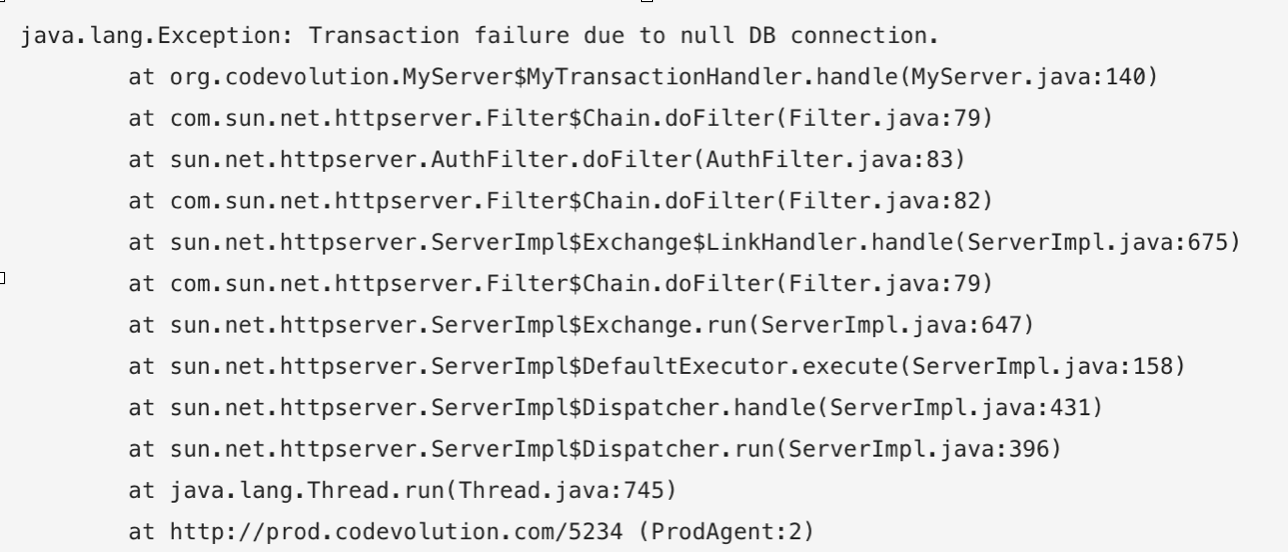
\includegraphics[width=\textwidth]{stack-with-link.png} 
    \begin{itemize}
  \item Are they locally defined?
  \item Are they static variables? 
  \item Are they arrays?
  \item Are they objects?
\end{itemize}


  \caption[Stack-trace with portal dashboard link]{Notice the link at the bottom of the stack.}
\end{figure}

This is currently achieved by adding an additional java.lang.StackTraceElement entry into the stack-trace. There are a few alternatives through which this can be implemented less intrusively, but this implementation was sufficient for all intents and purposes of this MVP, guaranteeing that any logging system which would record the stack-trace would also pick-up the URL to where it can be viewed in the Dashboard.

\subsubsection{Operating System specific code}
Compiler defined constants were used to customise the behaviour of the agent based on the operating system it is compiled for \cite{compiler}.

Two of the most important operating system specific parts were the threading library (windows.h vs pthread.h) and the JDK (win32 vs darwin).

\subsubsection{Building pipeline}
A few small scripts drive the building pipeline which quickly and predictably builds the Agent into libraries for different operating systems (.dylib, .dll and .so).

Moreover, the pipeline also takes care of building the test Java app used to assess the behaviour of the agent.


\subsection{API}
\subsubsection{Overview}
The API engine was built in Scala v2.11.8 using the Spray v1.3.3 Library for handling HTTP requests and the SBT tool for dependency management.

The ReactiveMongo v0.11.14 library provided the adaptor for communicating with the MongoDB database.

The codebase has been split into three main parts
\begin{itemize}
  \item Models, which are Scala objects and their writers and readers for conversion to JSON and to/from Mongo. Examples: User, UserApp, Log
  \item Providers, which interact with Mongo to obtain data. There generally is one provider for each Mongo collection used by the API. examples: UserProvider, LogProvider, AppProvider 
  \item Services, which define groups of request routes for different behaviours such the group handling authentication and the group handling app log submission and retrieval requests.
\end{itemize}


A quick look at the protocol used to communicate with the API from the point of view of the Agent and the Dashboard will be presented next.

\subsubsection{Agent app state messages}
There are three types of messages which represent the running state of an instance of an app.

The Start event can be accompanied by additional system properties data which could be used to differentiate between instances of the same app and provide additional debugging information in the Dashboard.

These messages are sent to the /log endpoint.

\begin{listing}[H]
\begin{minted}{xml}
    <app>
        <event>start</event>
        <hostname>My-MacBook-Pro.local</hostname>
        <pid>77764</pid>
        <command>./release/app.jar</command>
        <p_name>/usr/bin/java</p_name>
        <c_path>./release/app.jar</c_path>
        <jvm>Java HotSpot(TM) 64-Bit Server VM</jvm>
        <agentv>1.0.0</agentv>
    </app>
\end{minted}
\caption{XML start app message from agent to API}
\end{listing}



\begin{listing}[H]
\begin{minted}{xml}
    <app>
        <event>ping</event>
    </app>
\end{minted}
\caption{XML heartbeat message from agent to API}
\end{listing}



\begin{listing}[H]
\begin{minted}{xml}
    <app>
        <event>stop</event>
    </app>
\end{minted}
\caption{XML shutdown message from agent to API}
\end{listing}


\subsubsection{Agent log submit message}
This message contains the representation of an exception's details.

A few properties are recorded at the beginning, such as whether it has been caught or not, and if yes then by which method it is handled.  

A list of specifics for all the objects which were relevant to the stack trace follows (if they were found multiple times, they are recorded only once in this object list). Each entry contains the unique id, name, identified source, signature and value.

A final list, this time of stack-trace frames, completes the message. Each entry specifies the different variables the frame contains. If the variable was not an object, its value is specified right on the spot, otherwise it is cross-referenced to the object list.

These messages are sent to the /log endpoint.

\begin{listing}[H]
\begin{minted}{xml}
  <caught l="">
     <m><![CDATA[run]]></m>
     <sig><![CDATA[Lorg/codevolution/MyServer$1;]]></sig>
     <s><![CDATA[MyServer.java]]></s>
  </caught>
  <getMessage>
    <![CDATA[Manually thrown timer based custom exception]]>
  </getMessage>
  <objects>
     <v id="1447195560">
        <n>this</n>
        <s>Lorg/codevolution/MyServer$1;</s>
        <v><![CDATA[org.codevolution.MyServer$1@564273a8]]></v>
     </v>
  </objects>
  <sts>
     <st l="">
        <m><![CDATA[run]]></m>
        <sig><![CDATA[Lorg/codevolution/MyServer$1;]]></sig>
        <s><![CDATA[MyServer.java]]></s>
        <vars>
           <v>
              <n>testExceptionVar</n>
              <s>I</s>
              <v><![CDATA[5]]></v>
           </v>
           <v id="1447195560" />
        </vars>
     </st>
     <st l="">
        <m><![CDATA[mainLoop]]></m>
        <sig><![CDATA[Ljava/util/TimerThread;]]></sig>
        <s><![CDATA[Timer.java]]></s>
        <vars />
     </st>
     <st l="">
        <m><![CDATA[run]]></m>
        <sig><![CDATA[Ljava/util/TimerThread;]]></sig>
        <s><![CDATA[Timer.java]]></s>
        <vars />
     </st>
  </sts>
\end{minted}
\caption{XML stack-trace log message from agent to API}
\end{listing}




\subsubsection{Dashboard specific endpoints}

Multiple other endpoints exist such as those necessary for authentication, fetching user apps/stack-trace data, creating apps and registering accounts. It is beyond the scope of this report to go in-depth about them.

\subsection{Dashboard Portal}
\subsubsection{Overview}
Three main use cases were decided from the beginning drove the development of the dashboard:

\begin{itemize}
  \item User account - Account creation and session management
  \item Apps management - User apps view and app creation ability
  \item App management - Processed events list
  \item In-depth stack-trace - Log data exploration  
\end{itemize}

\subsubsection{Use case - User account}
\begin{figure}[H]
  \centering
    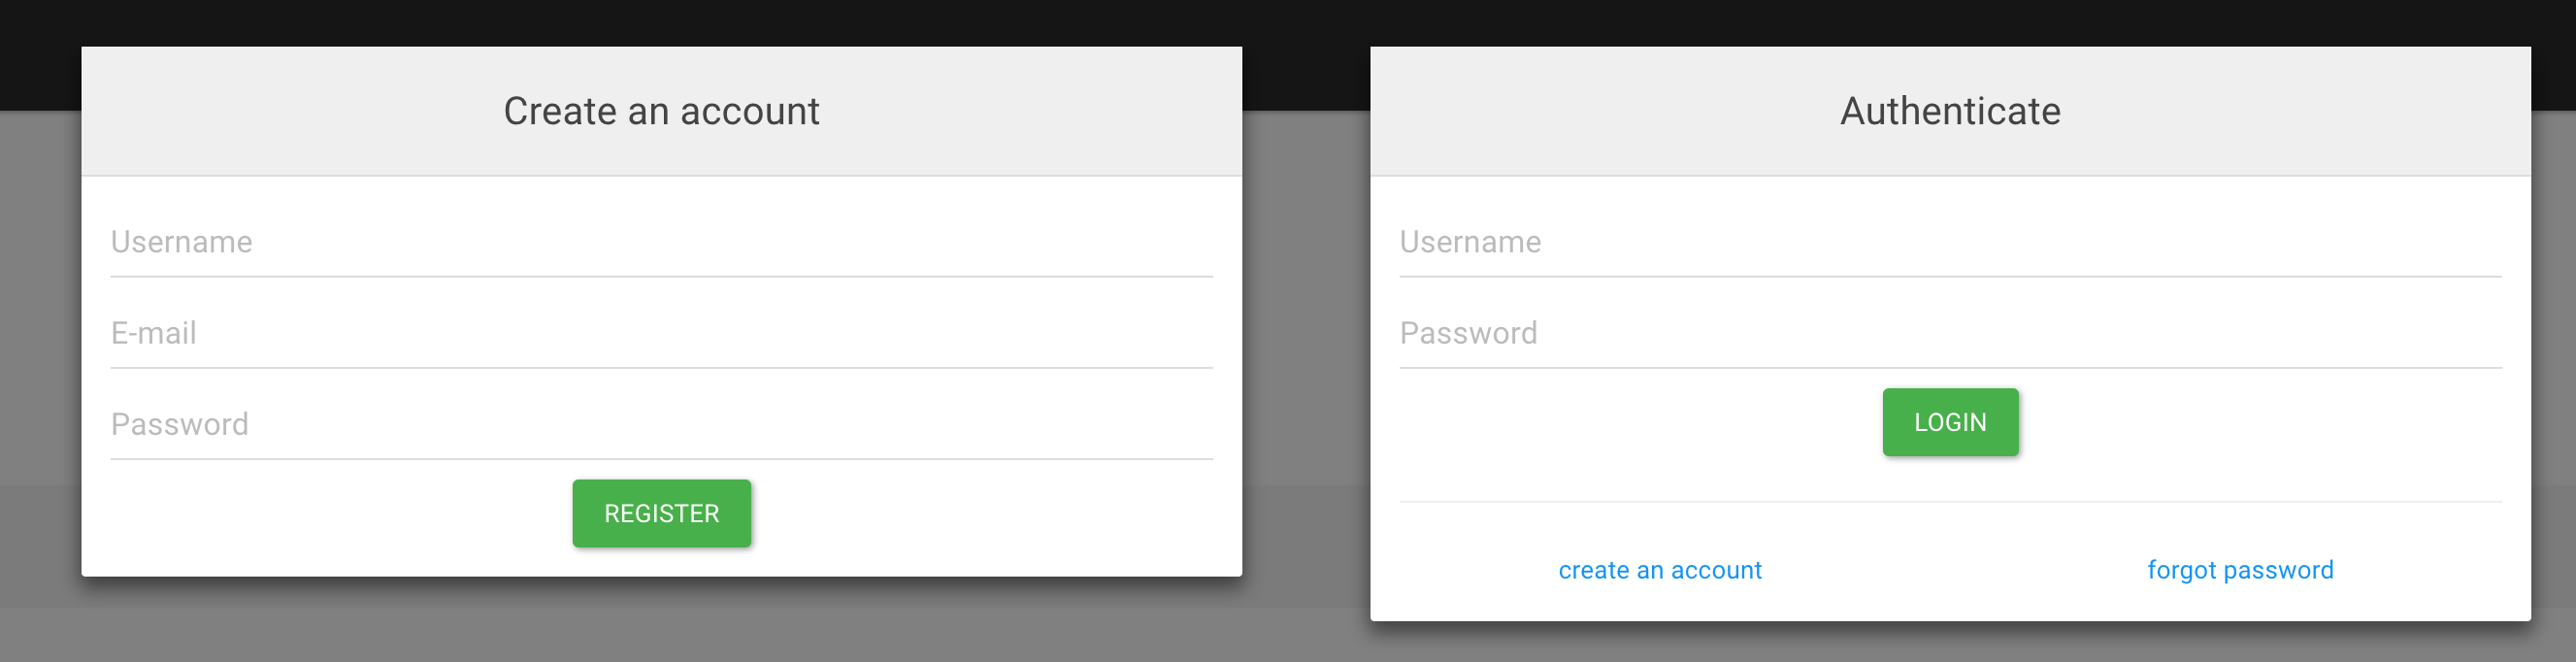
\includegraphics[width=\textwidth]{dashboard-account.png} 
  \caption[Dashboard - User account]{Dashboard - User account}
\end{figure}

The user can accomplish the task of authenticating on the Dashboard through the following
\begin{itemize}
  \item Quickly creating an account
  \item Using registration details to authenticate and explore data
\end{itemize}

\subsubsection{Use case - Apps management}
\begin{figure}[H]
  \centering
    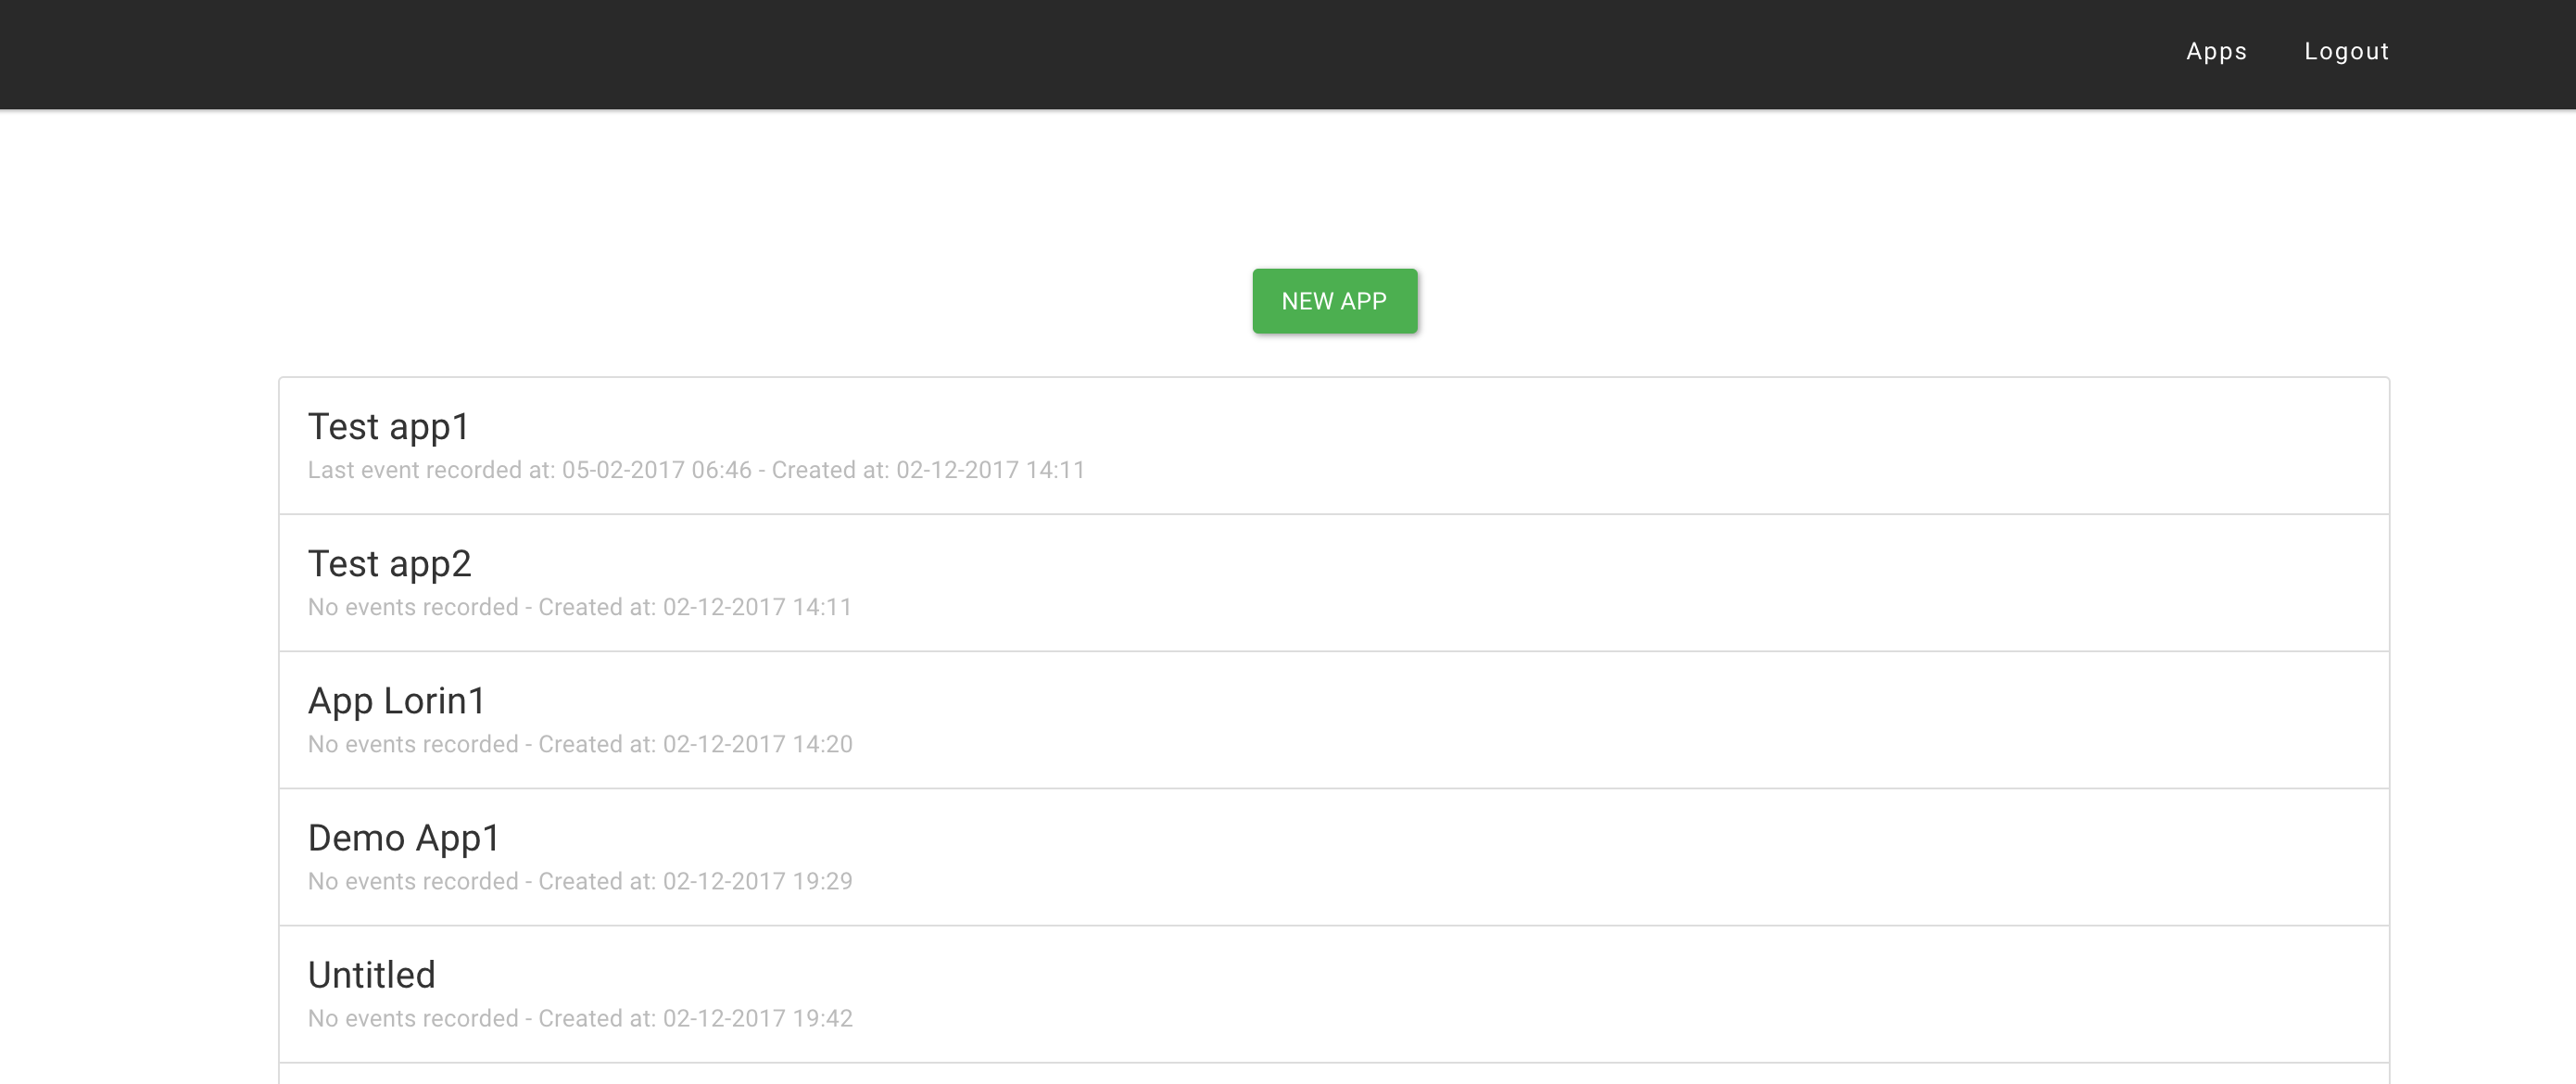
\includegraphics[width=\textwidth]{dashboard-apps.png} 
  \caption[Dashboard - Apps management]{Dashboard - Apps managements}
\end{figure}

The user can accomplish the task of managing his apps through the following
\begin{itemize}
    \item Creating a new app
  \item Viewing a list of created apps with the ability to move to a secondary in-depth view for each one
  \item Additional information provided for each app such as when the last even has come in
\end{itemize}

\subsubsection{Use case - User-app management}

\begin{figure}[H]
  \centering
    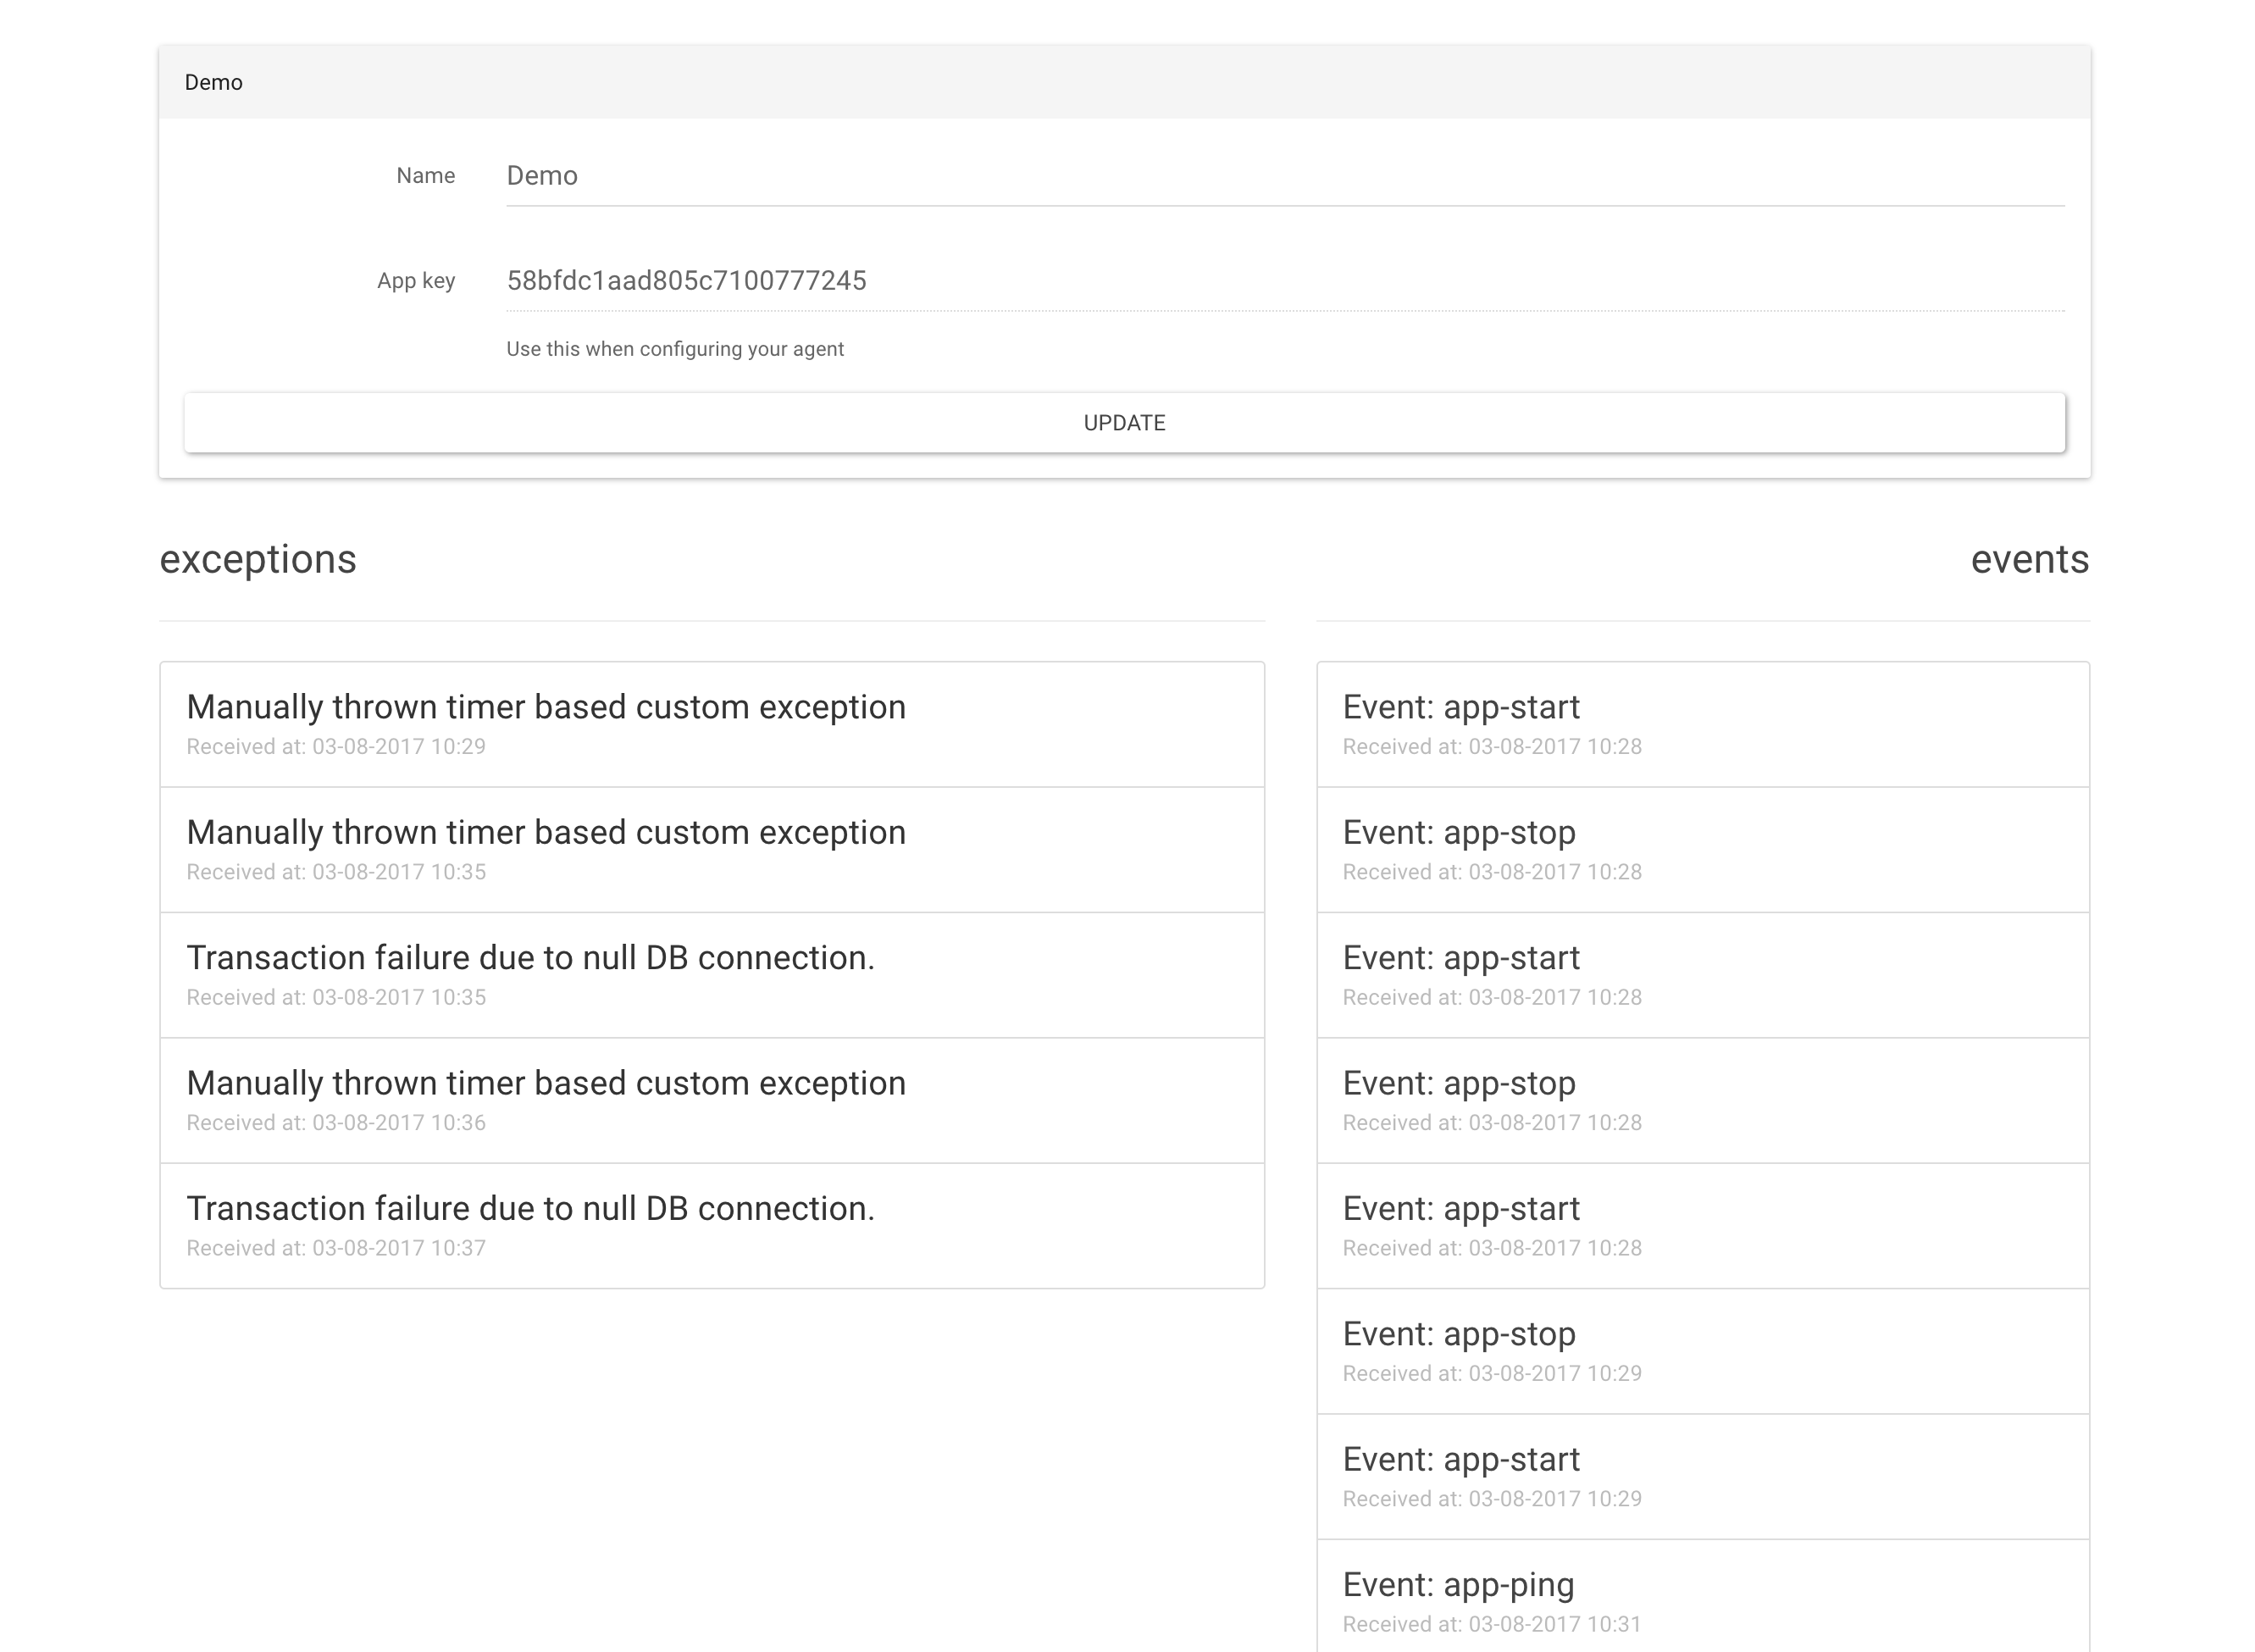
\includegraphics[width=\textwidth]{dashboard-app.png} 
  \caption[Dashboard - User-app management]{Dashboard - User-app management}
\end{figure}

The user can accomplish the task of managing his app through the following
\begin{itemize}
  \item Update basic details to customise the app configuration, such as its name
  \item Obtain the App key needed as an input to the Agent
  \item Explore recorded exceptions with the ability to move to a secondary in-depth view for each one
  \item View other events captured for the app such as the known start and shutdown times
\end{itemize}



\subsubsection{Use case - In-depth stack-trace view}

\begin{figure}[H]
  \centering
    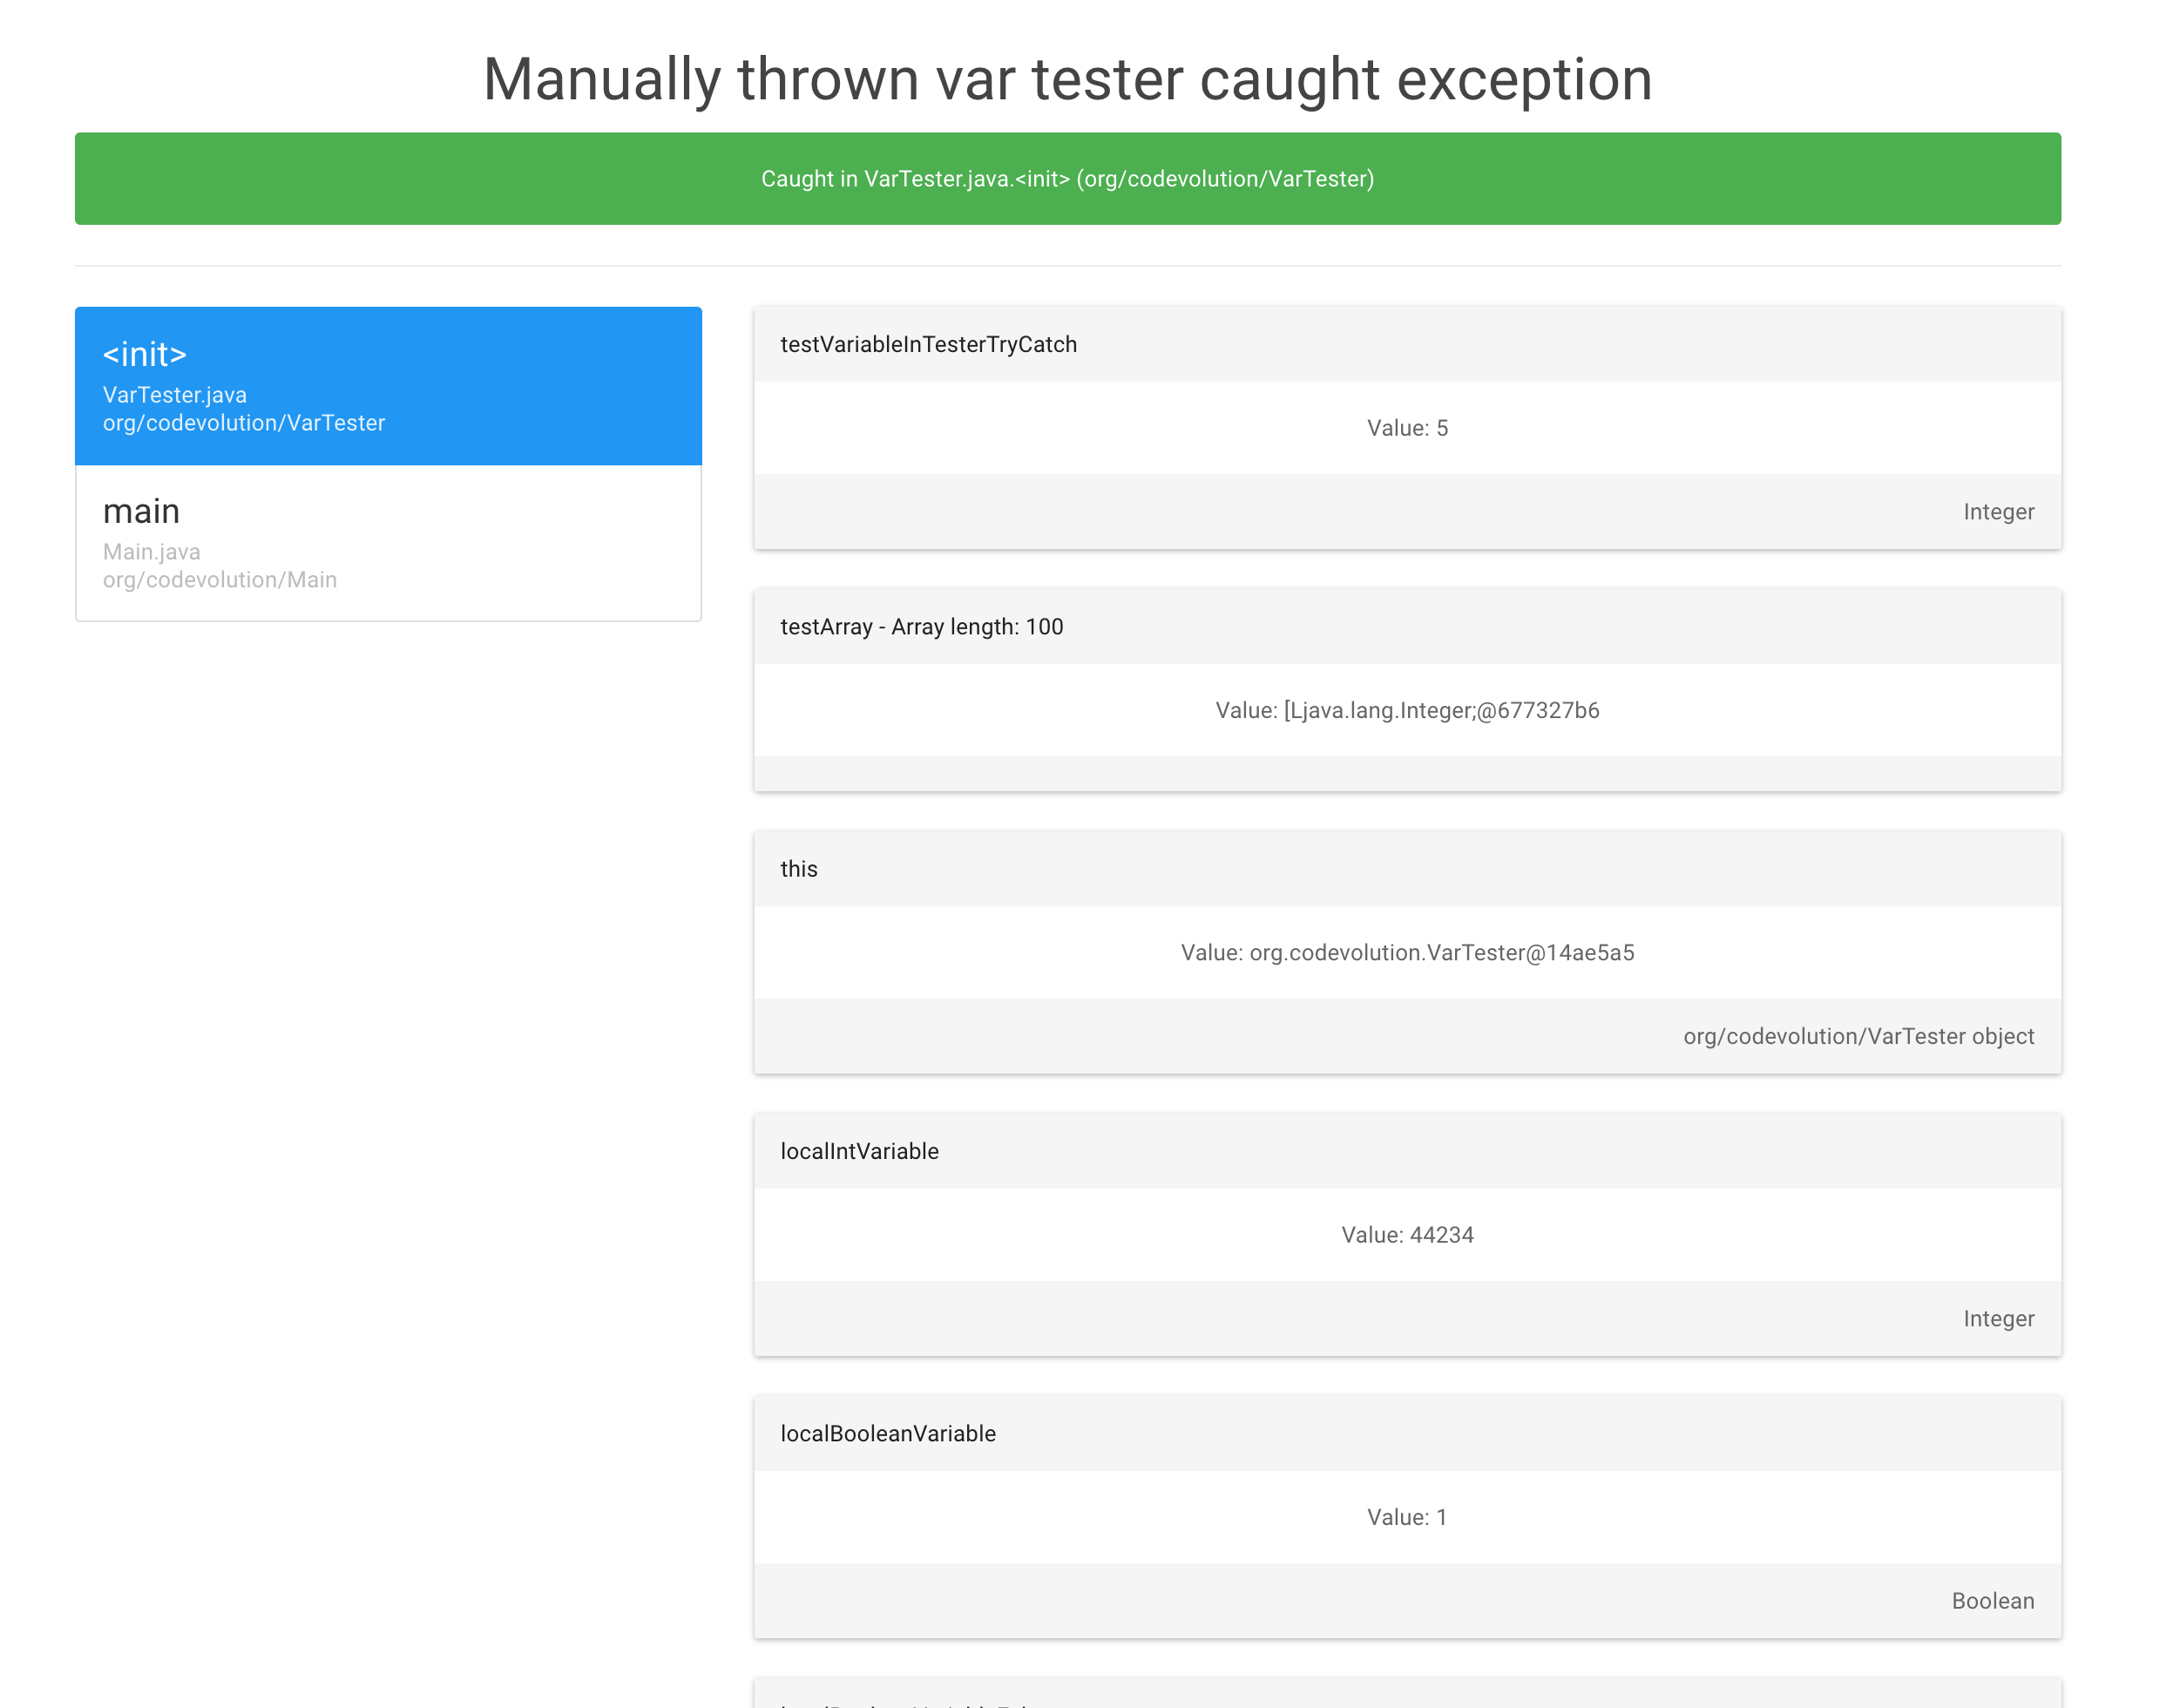
\includegraphics[width=\textwidth]{dashboard-exception.png} 
  \caption[Dashboard - In-depth stack-trace view]{Dashboard - In-depth stack-trace view}
\end{figure}

The XML stored for each stack-trace is parsed at this point in the controller of this view to then allow the view to match the variables inside the currently selected frame/method to the map of objects on a per-need basis. The format of the XML is explained in the Implementation section.

The user can accomplish the task of in-depth exploration of a recorded stack-trace through the following
\begin{itemize}
  \item Navigating from one frame of the stack-trace to another
  \item Visualising variables, with automatic mapping to human-readable types and values, per frame
  \item Availability of information on how the exception was handled app-side
\end{itemize}



\newpage

\section{Testing and evaluation}
\subsection{Overview}
A functional testing approach was taken as the main approach. 

A mock bank account management app has been setup using a simple Java web-server. The app was used for both testing and demonstration purposes.

A number of cases were implemented into the mock and expected the agent to handle:

\begin{itemize}
  \item Identify exceptions in other thread than the main one
  \item Identify exceptions driven by user input
  \item Deliver start/end and ping messages to the API
  \item Deliver exception logs to the API
  \item Correctly handle values of primitives and objects, statically and instance defined
  \item API engine unavailability
  \item Present a link to the Dashboard at the end of recorded stack-traces
\end{itemize}

\subsection{Agent testing and evaluation}
\subsubsection{Testing pipeline}
The main evaluation of the agent was done via the mock app. With each iteration of the agent, steps were taken to ensure this specific use-case was constantly fulfilled.

With every built attempt of the agent, if the built was successfully, the mock app would also be ran with the new agent attached.

\subsubsection{The mock Java bank account app}
The app uses a simple HttpServer setup, custom threads, timers and custom classes to assess and demonstrate the behaviour of the system

\begin{figure}[H]
  \centering
    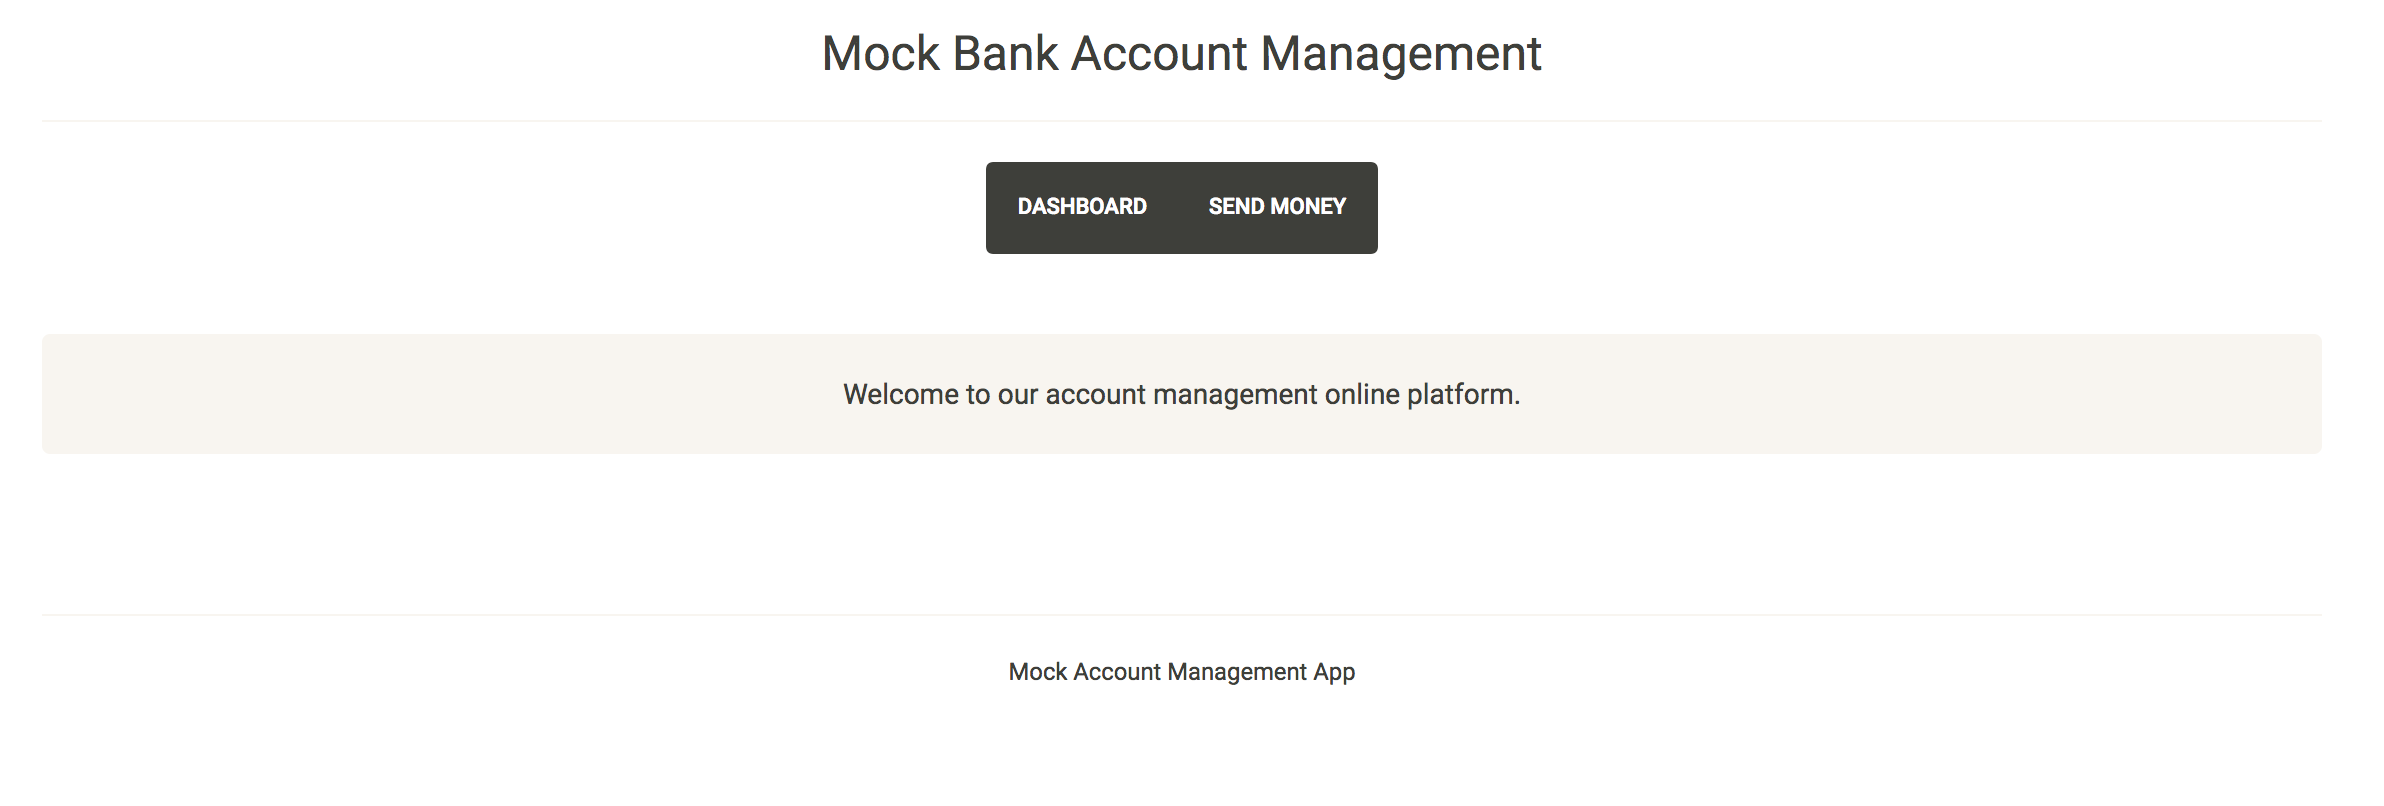
\includegraphics[width=\textwidth]{java-test.png}
  \caption[Mock bank account management app - Dashboard]{Mock bank account management app - Dashboard}
\end{figure}

\begin{figure}[H]
  \centering
    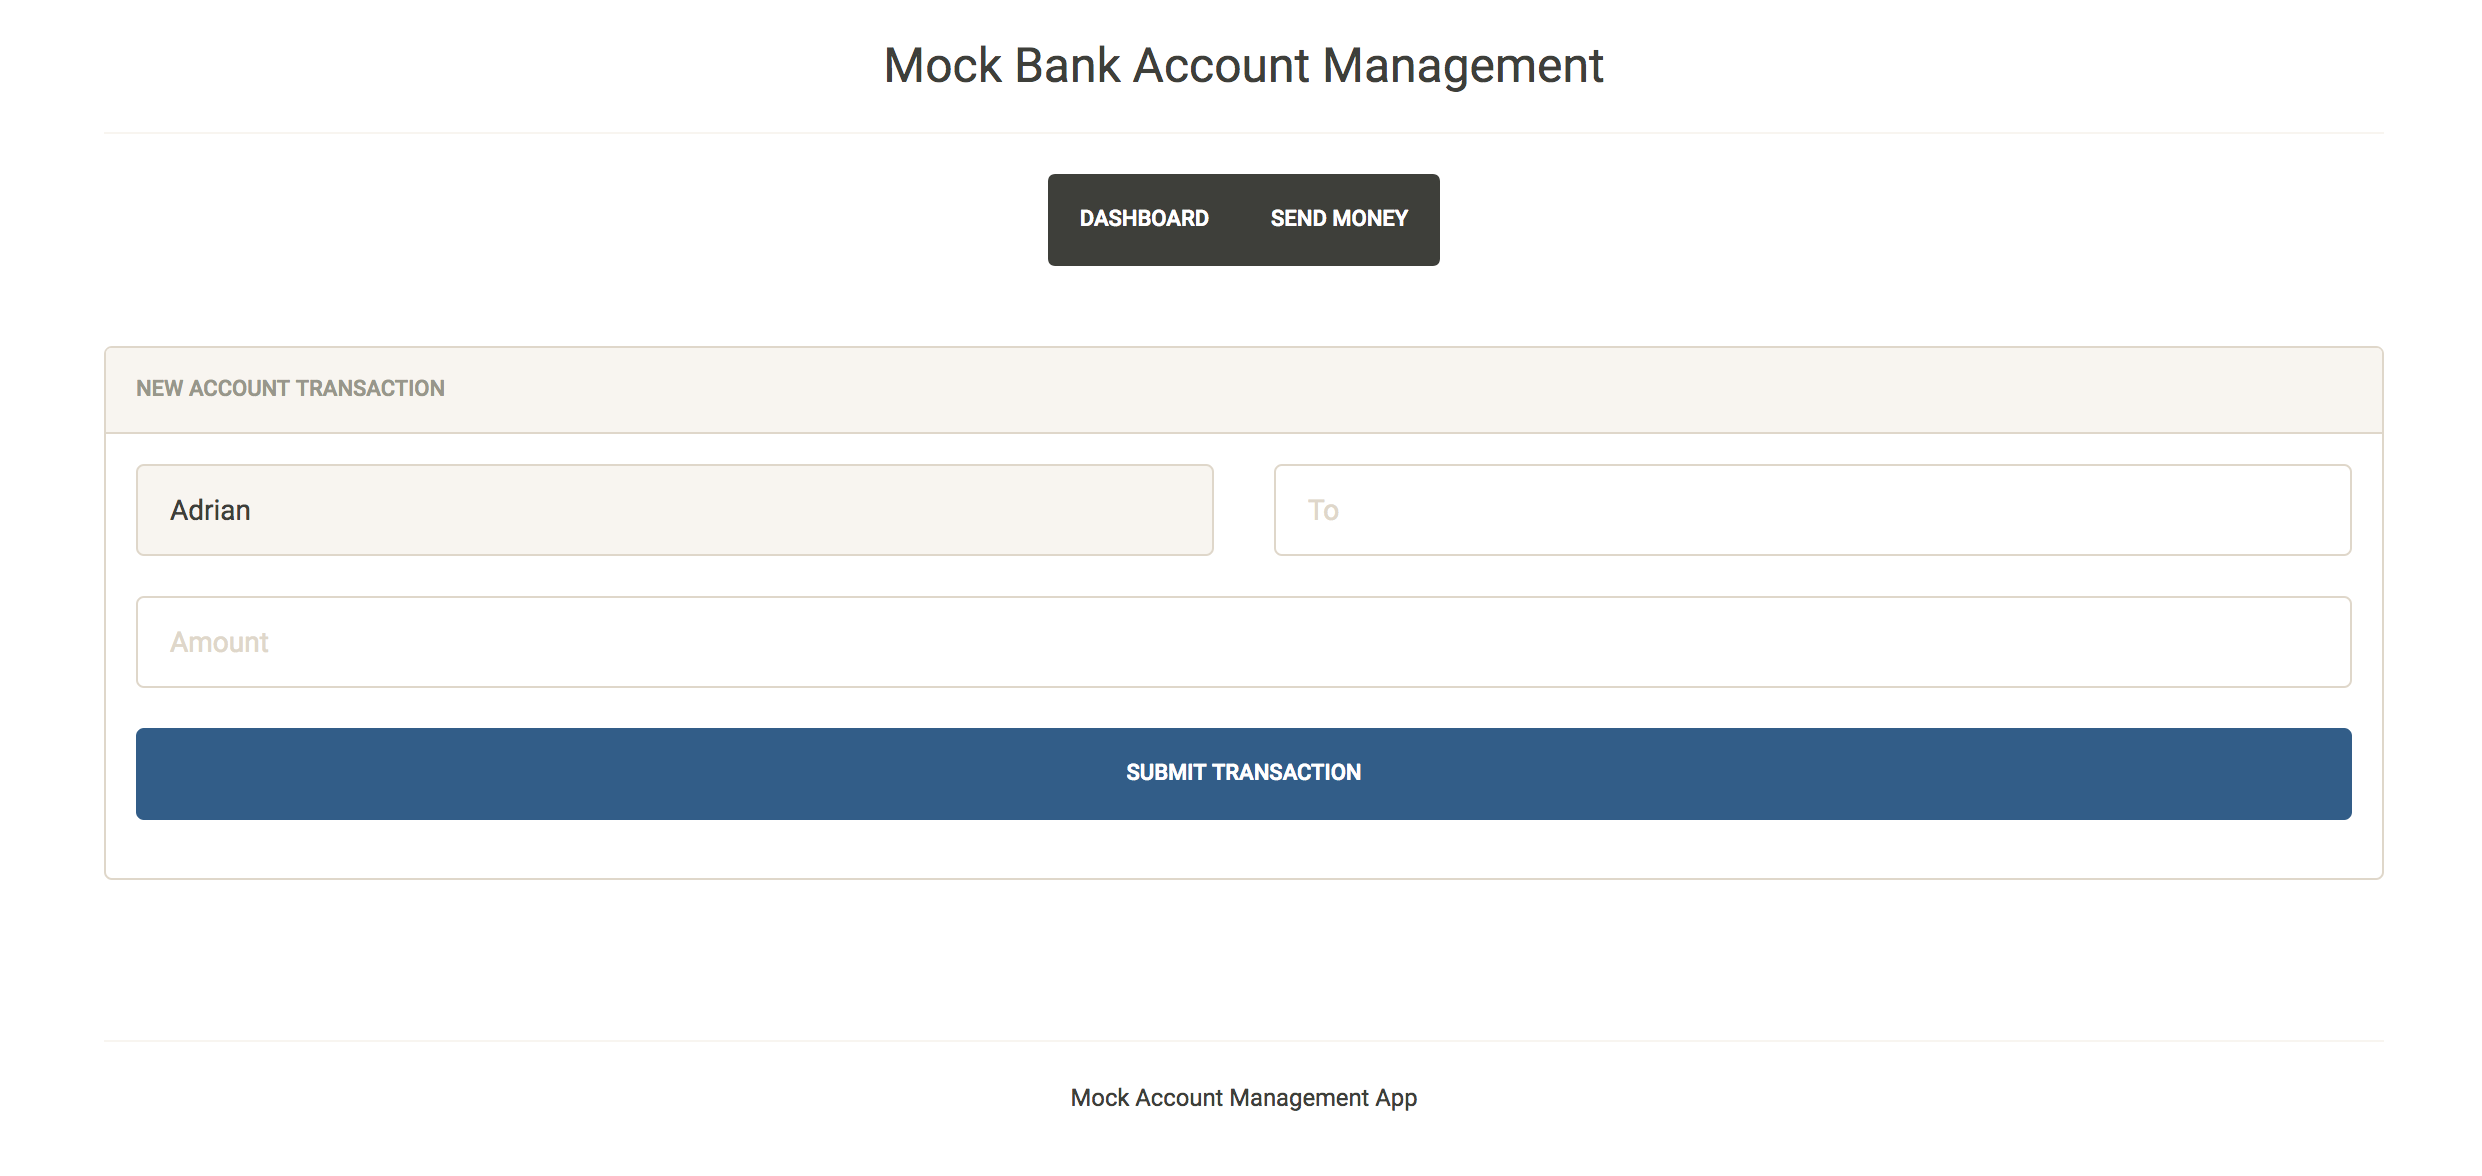
\includegraphics[width=\textwidth]{java-test2.png}
  \caption[Mock bank account management app - Submit transaction]{Mock bank account management app - Submit transaction}
\end{figure}

\begin{figure}[H]
  \centering
    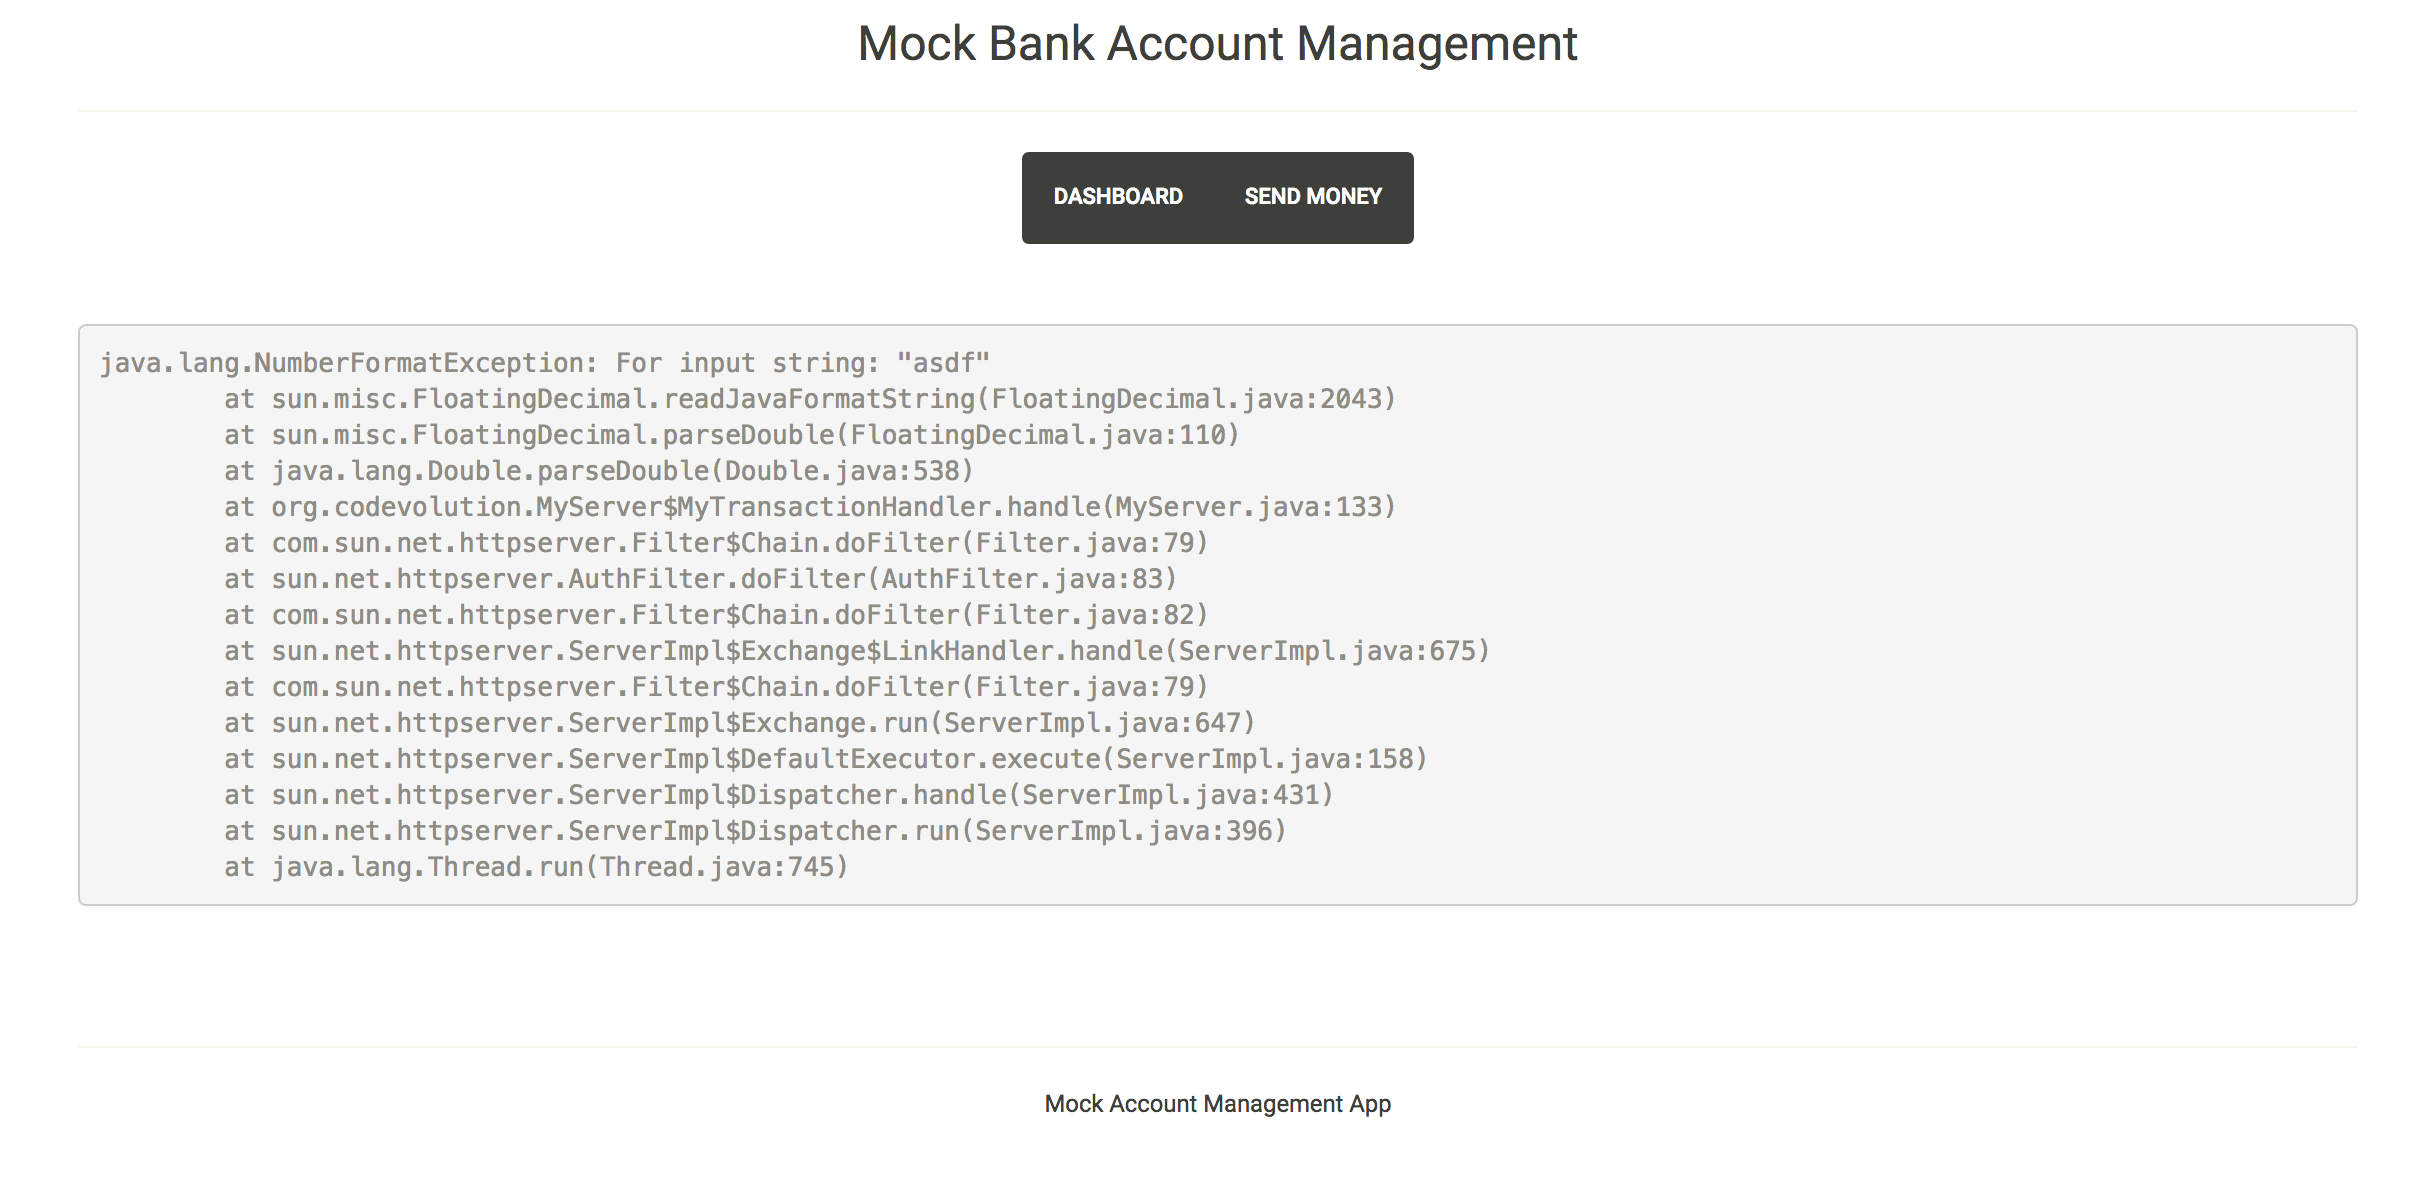
\includegraphics[width=\textwidth]{java-test3.png}
  \caption[Mock bank account management app - Exception]{Mock bank account management app - Exception}
\end{figure}

\subsection{Dashboard testing and evaluation}
This proved to be one of the most difficult parts to test as external testers would needs their agent to communicate to a server were an instance of the API engine would be running and one of the Dashboard.

Three students contributed by using the agent on their personal JVM-based apps and then employing the use of the dashboard to analyse the results.

An Amazon Web Service instance of the API engine and Dashboard were setup for this purpose and their use of the agent was done in both controlled  and uncontrolled environments.

\subsection{Operating systems}
The system was mostly tested using macOS Sierra driven machines with limited Windows testing.

The API engine was ran on macOS Sierra and Ubuntu 16 machines.

\subsection{Concluding remarks}
Given all the different components of the system, it proved hard to have all-around testing, especially due to the operating-system specific builds required for the agent component.

Moreover, finding external test users was challenging due to the technical learning curve needed to use the agent and the high level of system reliability required even for basic usage.


\newpage

\section{Conclusions}
\subsection{Limitations}
There was only so much the agent can do based on the requirement of having a low footprint. A cap on CPU and memory usage has not been implemented but would be necessary. 

\subsection{Testing}
Having multiple components, cross-operating system specifics and a bit of a learning curve required on the side of testers made the overall implementation harder to test and required more time to identify and rectify issues.

\subsection{Room for improvement}

\subsubsection{Multiple instances of the same app}
A mechanism could be setup to handle multiple recurrences of the same stack-traces so that they are not recorded multiple times (such as computing an unique hash based on the contents of the trace).

Agents could communicate to each other on the local network and share information about captured exception so as to avoid unnecessary processing being done.

\subsubsection{Code overlay - in progress}
For maximum efficacy, the dashboard should be able to display the code of every method on the stack-trace with an overlay of variable values on it.

There are multiple concerns with this approach which is why the implementation of this feature has been halted to make room for other critical parts.

How would the code-base be obtained? The agent has some code to handle directory parsing and looking into .Jar files. Research has been done into disassembling .class files and native libraries which could accomplish this. However, the complexity of an automated system which could handle this process was considered beyond the current scope of the project.

Also, once obtained, the code-base must be kept in an encrypted format and decrypted inside the user browser potentially using the same key which could be used for encrypting the variable data.

\subsubsection{Resource capping}
Limits should be imposed on the size of the heap that is to be recorded.

\subsubsection{Ignoring framework-specific code}

Stack-traces will most of the time very likely include methods which are not of interest, such as the ones of the framework we might be using (Spring, etc).

\subsubsection{Data Compression - in progress}

Miniz \cite{miniz} is a loss-less and quick data compression library coded in a single source file. This brings a low footprint on the agent library and reduces the bandwidth usage and increases speed at which data would be transferred from the agent to the API and between agent instances.

It is compiled as part of the agent code-base but full implementation was not achieved.

\subsubsection{Encryption}
AES256 encryption was supposed to be used to encrypt the variable date inside the agent before sending it to the storage system via the API. The key would have been stored locally and generated by the user.

The openssl library was meant to serve the native agent side of cryption \cite{openssl}.

The dashboard's Javascript library would have then used the same local key to decrypt the data once it safely arrived from the storage system, through the API, into the user's local browser and hence memory. This library was supposed to be used on the client side \cite{cryptojs} which supports AES cryption.

In this manner, the captured data would be readable only to key-holders.

\subsection{Concluding remarks}
The core of an utility for debugging JVMs in the described way was designed and built as a result of this project.

The tool has a built by developers for developers style, rendering it quite technical. This made it harder to test but brought more benefits to specialised end-users.

The JNI and JVMTI are powerful means to explore and manipulate the behaviour of JVMs and provide the means to develop advanced tools for both debugging and improving performance, this project being one of the many tools which could be developed using them.
\newpage



\section{References}

\printbibliography[title={~}]




\end{document}

